\section{Implementing a FIR Convolution filter}

\subsection{Linear, time-invariant systems}
For every possible input signal $x$, a system $H$ maps it to an output signal $H(x) = y$.

\begin{center}

\tikzset{every picture/.style={line width=0.75pt}} %set default line width to 0.75pt        

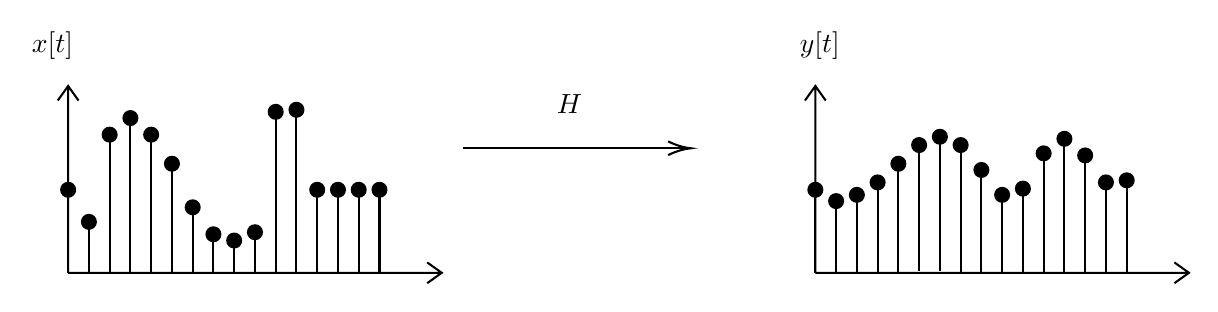
\begin{tikzpicture}[x=0.75pt,y=0.75pt,yscale=-1,xscale=1]
%uncomment if require: \path (0,300); %set diagram left start at 0, and has height of 300

%Shape: Axis 2D [id:dp7620621852352821] 
\draw  (70,170) -- (250,170)(70,80) -- (70,170) -- cycle (243,165) -- (250,170) -- (243,175) (65,87) -- (70,80) -- (75,87)  ;
%Straight Lines [id:da10165979286839177] 
\draw    (70,170) -- (70,130) ;
\draw [shift={(70,130)}, rotate = 270] [color={rgb, 255:red, 0; green, 0; blue, 0 }  ][fill={rgb, 255:red, 0; green, 0; blue, 0 }  ][line width=0.75]      (0, 0) circle [x radius= 3.35, y radius= 3.35]   ;
%Straight Lines [id:da39683654735642937] 
\draw    (260,110) -- (368,110) ;
\draw [shift={(370,110)}, rotate = 180] [color={rgb, 255:red, 0; green, 0; blue, 0 }  ][line width=0.75]    (10.93,-3.29) .. controls (6.95,-1.4) and (3.31,-0.3) .. (0,0) .. controls (3.31,0.3) and (6.95,1.4) .. (10.93,3.29)   ;
%Straight Lines [id:da44924365735005733] 
\draw    (80,170) -- (80,145.45) ;
\draw [shift={(80,145.45)}, rotate = 270] [color={rgb, 255:red, 0; green, 0; blue, 0 }  ][fill={rgb, 255:red, 0; green, 0; blue, 0 }  ][line width=0.75]      (0, 0) circle [x radius= 3.35, y radius= 3.35]   ;
%Straight Lines [id:da7890968080449057] 
\draw    (90,170) -- (90,103.45) ;
\draw [shift={(90,103.45)}, rotate = 270] [color={rgb, 255:red, 0; green, 0; blue, 0 }  ][fill={rgb, 255:red, 0; green, 0; blue, 0 }  ][line width=0.75]      (0, 0) circle [x radius= 3.35, y radius= 3.35]   ;
%Straight Lines [id:da773508268233024] 
\draw    (100,170) -- (100,95.45) ;
\draw [shift={(100,95.45)}, rotate = 270] [color={rgb, 255:red, 0; green, 0; blue, 0 }  ][fill={rgb, 255:red, 0; green, 0; blue, 0 }  ][line width=0.75]      (0, 0) circle [x radius= 3.35, y radius= 3.35]   ;
%Straight Lines [id:da6567081038357468] 
\draw    (110,170) -- (110,103.45) ;
\draw [shift={(110,103.45)}, rotate = 270] [color={rgb, 255:red, 0; green, 0; blue, 0 }  ][fill={rgb, 255:red, 0; green, 0; blue, 0 }  ][line width=0.75]      (0, 0) circle [x radius= 3.35, y radius= 3.35]   ;
%Straight Lines [id:da9418146736045092] 
\draw    (120,170) -- (120,117.45) ;
\draw [shift={(120,117.45)}, rotate = 270] [color={rgb, 255:red, 0; green, 0; blue, 0 }  ][fill={rgb, 255:red, 0; green, 0; blue, 0 }  ][line width=0.75]      (0, 0) circle [x radius= 3.35, y radius= 3.35]   ;
%Straight Lines [id:da4317568396628758] 
\draw    (130,170) -- (130,138.45) ;
\draw [shift={(130,138.45)}, rotate = 270] [color={rgb, 255:red, 0; green, 0; blue, 0 }  ][fill={rgb, 255:red, 0; green, 0; blue, 0 }  ][line width=0.75]      (0, 0) circle [x radius= 3.35, y radius= 3.35]   ;
%Straight Lines [id:da3454927320163593] 
\draw    (140,170) -- (140,151.45) ;
\draw [shift={(140,151.45)}, rotate = 270] [color={rgb, 255:red, 0; green, 0; blue, 0 }  ][fill={rgb, 255:red, 0; green, 0; blue, 0 }  ][line width=0.75]      (0, 0) circle [x radius= 3.35, y radius= 3.35]   ;
%Straight Lines [id:da8012366690435773] 
\draw    (150,170) -- (150,154.45) ;
\draw [shift={(150,154.45)}, rotate = 270] [color={rgb, 255:red, 0; green, 0; blue, 0 }  ][fill={rgb, 255:red, 0; green, 0; blue, 0 }  ][line width=0.75]      (0, 0) circle [x radius= 3.35, y radius= 3.35]   ;
%Straight Lines [id:da7481132266069989] 
\draw    (160,170) -- (160,150.45) ;
\draw [shift={(160,150.45)}, rotate = 270] [color={rgb, 255:red, 0; green, 0; blue, 0 }  ][fill={rgb, 255:red, 0; green, 0; blue, 0 }  ][line width=0.75]      (0, 0) circle [x radius= 3.35, y radius= 3.35]   ;
%Straight Lines [id:da5851003137414529] 
\draw    (170,170) -- (170,92.45) ;
\draw [shift={(170,92.45)}, rotate = 270] [color={rgb, 255:red, 0; green, 0; blue, 0 }  ][fill={rgb, 255:red, 0; green, 0; blue, 0 }  ][line width=0.75]      (0, 0) circle [x radius= 3.35, y radius= 3.35]   ;
%Straight Lines [id:da06689581831864433] 
\draw    (180,170) -- (180,91.45) ;
\draw [shift={(180,91.45)}, rotate = 270] [color={rgb, 255:red, 0; green, 0; blue, 0 }  ][fill={rgb, 255:red, 0; green, 0; blue, 0 }  ][line width=0.75]      (0, 0) circle [x radius= 3.35, y radius= 3.35]   ;
%Straight Lines [id:da3129227933038331] 
\draw    (190,170) -- (190,130) ;
\draw [shift={(190,130)}, rotate = 270] [color={rgb, 255:red, 0; green, 0; blue, 0 }  ][fill={rgb, 255:red, 0; green, 0; blue, 0 }  ][line width=0.75]      (0, 0) circle [x radius= 3.35, y radius= 3.35]   ;
%Straight Lines [id:da9555519859670675] 
\draw    (200,170) -- (200,130) ;
\draw [shift={(200,130)}, rotate = 270] [color={rgb, 255:red, 0; green, 0; blue, 0 }  ][fill={rgb, 255:red, 0; green, 0; blue, 0 }  ][line width=0.75]      (0, 0) circle [x radius= 3.35, y radius= 3.35]   ;
%Straight Lines [id:da04077313346769451] 
\draw    (210,170) -- (210,130) ;
\draw [shift={(210,130)}, rotate = 270] [color={rgb, 255:red, 0; green, 0; blue, 0 }  ][fill={rgb, 255:red, 0; green, 0; blue, 0 }  ][line width=0.75]      (0, 0) circle [x radius= 3.35, y radius= 3.35]   ;
%Straight Lines [id:da11417970555326062] 
\draw    (220,170) -- (220,130) ;
\draw [shift={(220,130)}, rotate = 270] [color={rgb, 255:red, 0; green, 0; blue, 0 }  ][fill={rgb, 255:red, 0; green, 0; blue, 0 }  ][line width=0.75]      (0, 0) circle [x radius= 3.35, y radius= 3.35]   ;
%Shape: Axis 2D [id:dp9161414698670188] 
\draw  (430,170) -- (610,170)(430,80) -- (430,170) -- cycle (603,165) -- (610,170) -- (603,175) (425,87) -- (430,80) -- (435,87)  ;
%Straight Lines [id:da5968862416413843] 
\draw    (430,170) -- (430,130) ;
\draw [shift={(430,130)}, rotate = 270] [color={rgb, 255:red, 0; green, 0; blue, 0 }  ][fill={rgb, 255:red, 0; green, 0; blue, 0 }  ][line width=0.75]      (0, 0) circle [x radius= 3.35, y radius= 3.35]   ;
%Straight Lines [id:da4691034609425129] 
\draw    (440,170) -- (440,135.45) ;
\draw [shift={(440,135.45)}, rotate = 270] [color={rgb, 255:red, 0; green, 0; blue, 0 }  ][fill={rgb, 255:red, 0; green, 0; blue, 0 }  ][line width=0.75]      (0, 0) circle [x radius= 3.35, y radius= 3.35]   ;
%Straight Lines [id:da09551995597622553] 
\draw    (450,170) -- (450,132.45) ;
\draw [shift={(450,132.45)}, rotate = 270] [color={rgb, 255:red, 0; green, 0; blue, 0 }  ][fill={rgb, 255:red, 0; green, 0; blue, 0 }  ][line width=0.75]      (0, 0) circle [x radius= 3.35, y radius= 3.35]   ;
%Straight Lines [id:da5740949302214927] 
\draw    (460,170) -- (460,126.45) ;
\draw [shift={(460,126.45)}, rotate = 270] [color={rgb, 255:red, 0; green, 0; blue, 0 }  ][fill={rgb, 255:red, 0; green, 0; blue, 0 }  ][line width=0.75]      (0, 0) circle [x radius= 3.35, y radius= 3.35]   ;
%Straight Lines [id:da39075441348314643] 
\draw    (470,170) -- (470,117.45) ;
\draw [shift={(470,117.45)}, rotate = 270] [color={rgb, 255:red, 0; green, 0; blue, 0 }  ][fill={rgb, 255:red, 0; green, 0; blue, 0 }  ][line width=0.75]      (0, 0) circle [x radius= 3.35, y radius= 3.35]   ;
%Straight Lines [id:da013782745620506964] 
\draw    (480,169) -- (480,108.45) ;
\draw [shift={(480,108.45)}, rotate = 270] [color={rgb, 255:red, 0; green, 0; blue, 0 }  ][fill={rgb, 255:red, 0; green, 0; blue, 0 }  ][line width=0.75]      (0, 0) circle [x radius= 3.35, y radius= 3.35]   ;
%Straight Lines [id:da023189974427857085] 
\draw    (490,169) -- (490,104.45) ;
\draw [shift={(490,104.45)}, rotate = 270] [color={rgb, 255:red, 0; green, 0; blue, 0 }  ][fill={rgb, 255:red, 0; green, 0; blue, 0 }  ][line width=0.75]      (0, 0) circle [x radius= 3.35, y radius= 3.35]   ;
%Straight Lines [id:da9559962538529173] 
\draw    (500,170) -- (500,108.45) ;
\draw [shift={(500,108.45)}, rotate = 270] [color={rgb, 255:red, 0; green, 0; blue, 0 }  ][fill={rgb, 255:red, 0; green, 0; blue, 0 }  ][line width=0.75]      (0, 0) circle [x radius= 3.35, y radius= 3.35]   ;
%Straight Lines [id:da5723716167474444] 
\draw    (510,170) -- (510,120.45) ;
\draw [shift={(510,120.45)}, rotate = 270] [color={rgb, 255:red, 0; green, 0; blue, 0 }  ][fill={rgb, 255:red, 0; green, 0; blue, 0 }  ][line width=0.75]      (0, 0) circle [x radius= 3.35, y radius= 3.35]   ;
%Straight Lines [id:da7499000798069754] 
\draw    (520,170) -- (520,132.45) ;
\draw [shift={(520,132.45)}, rotate = 270] [color={rgb, 255:red, 0; green, 0; blue, 0 }  ][fill={rgb, 255:red, 0; green, 0; blue, 0 }  ][line width=0.75]      (0, 0) circle [x radius= 3.35, y radius= 3.35]   ;
%Straight Lines [id:da5416941952503426] 
\draw    (530,170) -- (530,129.45) ;
\draw [shift={(530,129.45)}, rotate = 270] [color={rgb, 255:red, 0; green, 0; blue, 0 }  ][fill={rgb, 255:red, 0; green, 0; blue, 0 }  ][line width=0.75]      (0, 0) circle [x radius= 3.35, y radius= 3.35]   ;
%Straight Lines [id:da10267025145778486] 
\draw    (540,170) -- (540,112.45) ;
\draw [shift={(540,112.45)}, rotate = 270] [color={rgb, 255:red, 0; green, 0; blue, 0 }  ][fill={rgb, 255:red, 0; green, 0; blue, 0 }  ][line width=0.75]      (0, 0) circle [x radius= 3.35, y radius= 3.35]   ;
%Straight Lines [id:da25612849585496567] 
\draw    (550,170) -- (550,105.45) ;
\draw [shift={(550,105.45)}, rotate = 270] [color={rgb, 255:red, 0; green, 0; blue, 0 }  ][fill={rgb, 255:red, 0; green, 0; blue, 0 }  ][line width=0.75]      (0, 0) circle [x radius= 3.35, y radius= 3.35]   ;
%Straight Lines [id:da6464072175044743] 
\draw    (560,170) -- (560,113.45) ;
\draw [shift={(560,113.45)}, rotate = 270] [color={rgb, 255:red, 0; green, 0; blue, 0 }  ][fill={rgb, 255:red, 0; green, 0; blue, 0 }  ][line width=0.75]      (0, 0) circle [x radius= 3.35, y radius= 3.35]   ;
%Straight Lines [id:da8964188711628558] 
\draw    (570,170) -- (570,126.45) ;
\draw [shift={(570,126.45)}, rotate = 270] [color={rgb, 255:red, 0; green, 0; blue, 0 }  ][fill={rgb, 255:red, 0; green, 0; blue, 0 }  ][line width=0.75]      (0, 0) circle [x radius= 3.35, y radius= 3.35]   ;
%Straight Lines [id:da48746996903225936] 
\draw    (580,170) -- (580,125.45) ;
\draw [shift={(580,125.45)}, rotate = 270] [color={rgb, 255:red, 0; green, 0; blue, 0 }  ][fill={rgb, 255:red, 0; green, 0; blue, 0 }  ][line width=0.75]      (0, 0) circle [x radius= 3.35, y radius= 3.35]   ;

% Text Node
\draw (51,52.4) node [anchor=north west][inner sep=0.75pt]    {$x[ t]$};
% Text Node
\draw (421,52.4) node [anchor=north west][inner sep=0.75pt]    {$y[ t]$};
% Text Node
\draw (304,82.4) node [anchor=north west][inner sep=0.75pt]    {$H$};


\end{tikzpicture}
\end{center}
A linear system is one which satisfies the superposition and scaling properties:

\textbf{Superposition property:}\\
A system $H$ satisfies the superposition property if applying the system to a sum
of two signals $x_1$ and $x_2$ is equivalent to applying the system to the two signals,
and then summing the results.
$$H(x_1 + x_2) = H(x_1) + H(x_2)$$

\textbf{Scaling Property:}\\
A system $H$ satisfies the scaling property if applying a system to a signal that is scaled by a factor
is equivalent to first applying the system to the signal and then scaling the result by that factor.
$$H(\lambda x_1) = \lambda H(x_1)$$


\textbf{Time-invariance property:}\\
A system is time invariant if shifting the input signal in time and then
applying the system gives an output equivalent to if you first apply the system, 
and then shift the result in time.

\begin{center}

\tikzset{every picture/.style={line width=0.75pt}} %set default line width to 0.75pt        

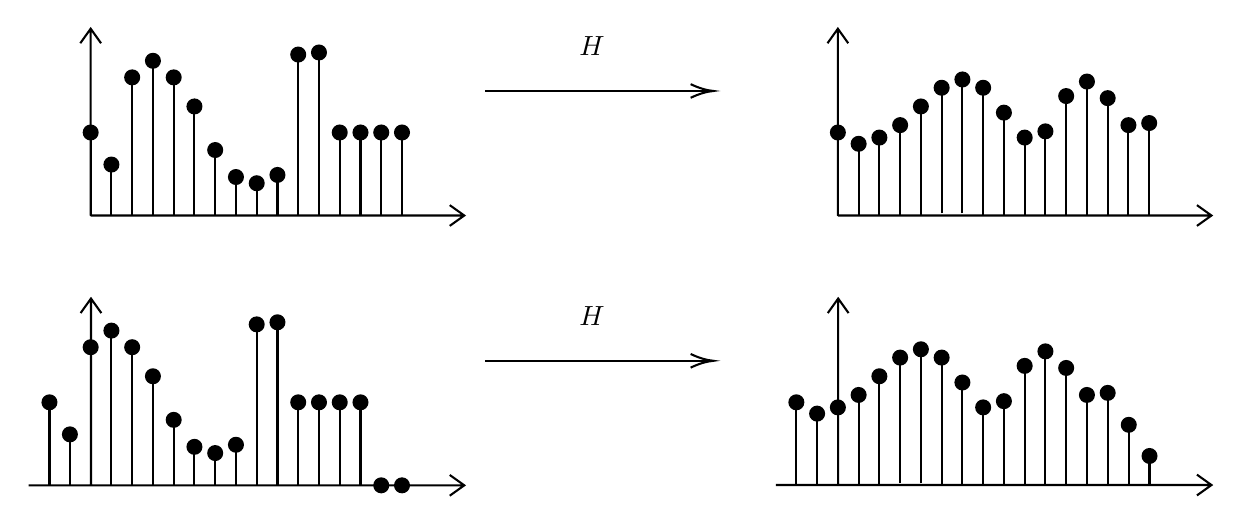
\begin{tikzpicture}[x=0.75pt,y=0.75pt,yscale=-1,xscale=1]
%uncomment if require: \path (0,355); %set diagram left start at 0, and has height of 355

%Shape: Axis 2D [id:dp7620621852352821] 
\draw  (70,170) -- (250,170)(70,80) -- (70,170) -- cycle (243,165) -- (250,170) -- (243,175) (65,87) -- (70,80) -- (75,87)  ;
%Straight Lines [id:da10165979286839177] 
\draw    (70,170) -- (70,130) ;
\draw [shift={(70,130)}, rotate = 270] [color={rgb, 255:red, 0; green, 0; blue, 0 }  ][fill={rgb, 255:red, 0; green, 0; blue, 0 }  ][line width=0.75]      (0, 0) circle [x radius= 3.35, y radius= 3.35]   ;
%Straight Lines [id:da39683654735642937] 
\draw    (260,110) -- (368,110) ;
\draw [shift={(370,110)}, rotate = 180] [color={rgb, 255:red, 0; green, 0; blue, 0 }  ][line width=0.75]    (10.93,-3.29) .. controls (6.95,-1.4) and (3.31,-0.3) .. (0,0) .. controls (3.31,0.3) and (6.95,1.4) .. (10.93,3.29)   ;
%Straight Lines [id:da44924365735005733] 
\draw    (80,170) -- (80,145.45) ;
\draw [shift={(80,145.45)}, rotate = 270] [color={rgb, 255:red, 0; green, 0; blue, 0 }  ][fill={rgb, 255:red, 0; green, 0; blue, 0 }  ][line width=0.75]      (0, 0) circle [x radius= 3.35, y radius= 3.35]   ;
%Straight Lines [id:da7890968080449057] 
\draw    (90,170) -- (90,103.45) ;
\draw [shift={(90,103.45)}, rotate = 270] [color={rgb, 255:red, 0; green, 0; blue, 0 }  ][fill={rgb, 255:red, 0; green, 0; blue, 0 }  ][line width=0.75]      (0, 0) circle [x radius= 3.35, y radius= 3.35]   ;
%Straight Lines [id:da773508268233024] 
\draw    (100,170) -- (100,95.45) ;
\draw [shift={(100,95.45)}, rotate = 270] [color={rgb, 255:red, 0; green, 0; blue, 0 }  ][fill={rgb, 255:red, 0; green, 0; blue, 0 }  ][line width=0.75]      (0, 0) circle [x radius= 3.35, y radius= 3.35]   ;
%Straight Lines [id:da6567081038357468] 
\draw    (110,170) -- (110,103.45) ;
\draw [shift={(110,103.45)}, rotate = 270] [color={rgb, 255:red, 0; green, 0; blue, 0 }  ][fill={rgb, 255:red, 0; green, 0; blue, 0 }  ][line width=0.75]      (0, 0) circle [x radius= 3.35, y radius= 3.35]   ;
%Straight Lines [id:da9418146736045092] 
\draw    (120,170) -- (120,117.45) ;
\draw [shift={(120,117.45)}, rotate = 270] [color={rgb, 255:red, 0; green, 0; blue, 0 }  ][fill={rgb, 255:red, 0; green, 0; blue, 0 }  ][line width=0.75]      (0, 0) circle [x radius= 3.35, y radius= 3.35]   ;
%Straight Lines [id:da4317568396628758] 
\draw    (130,170) -- (130,138.45) ;
\draw [shift={(130,138.45)}, rotate = 270] [color={rgb, 255:red, 0; green, 0; blue, 0 }  ][fill={rgb, 255:red, 0; green, 0; blue, 0 }  ][line width=0.75]      (0, 0) circle [x radius= 3.35, y radius= 3.35]   ;
%Straight Lines [id:da3454927320163593] 
\draw    (140,170) -- (140,151.45) ;
\draw [shift={(140,151.45)}, rotate = 270] [color={rgb, 255:red, 0; green, 0; blue, 0 }  ][fill={rgb, 255:red, 0; green, 0; blue, 0 }  ][line width=0.75]      (0, 0) circle [x radius= 3.35, y radius= 3.35]   ;
%Straight Lines [id:da8012366690435773] 
\draw    (150,170) -- (150,154.45) ;
\draw [shift={(150,154.45)}, rotate = 270] [color={rgb, 255:red, 0; green, 0; blue, 0 }  ][fill={rgb, 255:red, 0; green, 0; blue, 0 }  ][line width=0.75]      (0, 0) circle [x radius= 3.35, y radius= 3.35]   ;
%Straight Lines [id:da7481132266069989] 
\draw    (160,170) -- (160,150.45) ;
\draw [shift={(160,150.45)}, rotate = 270] [color={rgb, 255:red, 0; green, 0; blue, 0 }  ][fill={rgb, 255:red, 0; green, 0; blue, 0 }  ][line width=0.75]      (0, 0) circle [x radius= 3.35, y radius= 3.35]   ;
%Straight Lines [id:da5851003137414529] 
\draw    (170,170) -- (170,92.45) ;
\draw [shift={(170,92.45)}, rotate = 270] [color={rgb, 255:red, 0; green, 0; blue, 0 }  ][fill={rgb, 255:red, 0; green, 0; blue, 0 }  ][line width=0.75]      (0, 0) circle [x radius= 3.35, y radius= 3.35]   ;
%Straight Lines [id:da06689581831864433] 
\draw    (180,170) -- (180,91.45) ;
\draw [shift={(180,91.45)}, rotate = 270] [color={rgb, 255:red, 0; green, 0; blue, 0 }  ][fill={rgb, 255:red, 0; green, 0; blue, 0 }  ][line width=0.75]      (0, 0) circle [x radius= 3.35, y radius= 3.35]   ;
%Straight Lines [id:da3129227933038331] 
\draw    (190,170) -- (190,130) ;
\draw [shift={(190,130)}, rotate = 270] [color={rgb, 255:red, 0; green, 0; blue, 0 }  ][fill={rgb, 255:red, 0; green, 0; blue, 0 }  ][line width=0.75]      (0, 0) circle [x radius= 3.35, y radius= 3.35]   ;
%Straight Lines [id:da9555519859670675] 
\draw    (200,170) -- (200,130) ;
\draw [shift={(200,130)}, rotate = 270] [color={rgb, 255:red, 0; green, 0; blue, 0 }  ][fill={rgb, 255:red, 0; green, 0; blue, 0 }  ][line width=0.75]      (0, 0) circle [x radius= 3.35, y radius= 3.35]   ;
%Straight Lines [id:da04077313346769451] 
\draw    (210,170) -- (210,130) ;
\draw [shift={(210,130)}, rotate = 270] [color={rgb, 255:red, 0; green, 0; blue, 0 }  ][fill={rgb, 255:red, 0; green, 0; blue, 0 }  ][line width=0.75]      (0, 0) circle [x radius= 3.35, y radius= 3.35]   ;
%Straight Lines [id:da11417970555326062] 
\draw    (220,170) -- (220,130) ;
\draw [shift={(220,130)}, rotate = 270] [color={rgb, 255:red, 0; green, 0; blue, 0 }  ][fill={rgb, 255:red, 0; green, 0; blue, 0 }  ][line width=0.75]      (0, 0) circle [x radius= 3.35, y radius= 3.35]   ;
%Shape: Axis 2D [id:dp9161414698670188] 
\draw  (430,170) -- (610,170)(430,80) -- (430,170) -- cycle (603,165) -- (610,170) -- (603,175) (425,87) -- (430,80) -- (435,87)  ;
%Straight Lines [id:da5968862416413843] 
\draw    (430,170) -- (430,130) ;
\draw [shift={(430,130)}, rotate = 270] [color={rgb, 255:red, 0; green, 0; blue, 0 }  ][fill={rgb, 255:red, 0; green, 0; blue, 0 }  ][line width=0.75]      (0, 0) circle [x radius= 3.35, y radius= 3.35]   ;
%Straight Lines [id:da4691034609425129] 
\draw    (440,170) -- (440,135.45) ;
\draw [shift={(440,135.45)}, rotate = 270] [color={rgb, 255:red, 0; green, 0; blue, 0 }  ][fill={rgb, 255:red, 0; green, 0; blue, 0 }  ][line width=0.75]      (0, 0) circle [x radius= 3.35, y radius= 3.35]   ;
%Straight Lines [id:da09551995597622553] 
\draw    (450,170) -- (450,132.45) ;
\draw [shift={(450,132.45)}, rotate = 270] [color={rgb, 255:red, 0; green, 0; blue, 0 }  ][fill={rgb, 255:red, 0; green, 0; blue, 0 }  ][line width=0.75]      (0, 0) circle [x radius= 3.35, y radius= 3.35]   ;
%Straight Lines [id:da5740949302214927] 
\draw    (460,170) -- (460,126.45) ;
\draw [shift={(460,126.45)}, rotate = 270] [color={rgb, 255:red, 0; green, 0; blue, 0 }  ][fill={rgb, 255:red, 0; green, 0; blue, 0 }  ][line width=0.75]      (0, 0) circle [x radius= 3.35, y radius= 3.35]   ;
%Straight Lines [id:da39075441348314643] 
\draw    (470,170) -- (470,117.45) ;
\draw [shift={(470,117.45)}, rotate = 270] [color={rgb, 255:red, 0; green, 0; blue, 0 }  ][fill={rgb, 255:red, 0; green, 0; blue, 0 }  ][line width=0.75]      (0, 0) circle [x radius= 3.35, y radius= 3.35]   ;
%Straight Lines [id:da013782745620506964] 
\draw    (480,169) -- (480,108.45) ;
\draw [shift={(480,108.45)}, rotate = 270] [color={rgb, 255:red, 0; green, 0; blue, 0 }  ][fill={rgb, 255:red, 0; green, 0; blue, 0 }  ][line width=0.75]      (0, 0) circle [x radius= 3.35, y radius= 3.35]   ;
%Straight Lines [id:da023189974427857085] 
\draw    (490,169) -- (490,104.45) ;
\draw [shift={(490,104.45)}, rotate = 270] [color={rgb, 255:red, 0; green, 0; blue, 0 }  ][fill={rgb, 255:red, 0; green, 0; blue, 0 }  ][line width=0.75]      (0, 0) circle [x radius= 3.35, y radius= 3.35]   ;
%Straight Lines [id:da9559962538529173] 
\draw    (500,170) -- (500,108.45) ;
\draw [shift={(500,108.45)}, rotate = 270] [color={rgb, 255:red, 0; green, 0; blue, 0 }  ][fill={rgb, 255:red, 0; green, 0; blue, 0 }  ][line width=0.75]      (0, 0) circle [x radius= 3.35, y radius= 3.35]   ;
%Straight Lines [id:da5723716167474444] 
\draw    (510,170) -- (510,120.45) ;
\draw [shift={(510,120.45)}, rotate = 270] [color={rgb, 255:red, 0; green, 0; blue, 0 }  ][fill={rgb, 255:red, 0; green, 0; blue, 0 }  ][line width=0.75]      (0, 0) circle [x radius= 3.35, y radius= 3.35]   ;
%Straight Lines [id:da7499000798069754] 
\draw    (520,170) -- (520,132.45) ;
\draw [shift={(520,132.45)}, rotate = 270] [color={rgb, 255:red, 0; green, 0; blue, 0 }  ][fill={rgb, 255:red, 0; green, 0; blue, 0 }  ][line width=0.75]      (0, 0) circle [x radius= 3.35, y radius= 3.35]   ;
%Straight Lines [id:da5416941952503426] 
\draw    (530,170) -- (530,129.45) ;
\draw [shift={(530,129.45)}, rotate = 270] [color={rgb, 255:red, 0; green, 0; blue, 0 }  ][fill={rgb, 255:red, 0; green, 0; blue, 0 }  ][line width=0.75]      (0, 0) circle [x radius= 3.35, y radius= 3.35]   ;
%Straight Lines [id:da10267025145778486] 
\draw    (540,170) -- (540,112.45) ;
\draw [shift={(540,112.45)}, rotate = 270] [color={rgb, 255:red, 0; green, 0; blue, 0 }  ][fill={rgb, 255:red, 0; green, 0; blue, 0 }  ][line width=0.75]      (0, 0) circle [x radius= 3.35, y radius= 3.35]   ;
%Straight Lines [id:da25612849585496567] 
\draw    (550,170) -- (550,105.45) ;
\draw [shift={(550,105.45)}, rotate = 270] [color={rgb, 255:red, 0; green, 0; blue, 0 }  ][fill={rgb, 255:red, 0; green, 0; blue, 0 }  ][line width=0.75]      (0, 0) circle [x radius= 3.35, y radius= 3.35]   ;
%Straight Lines [id:da6464072175044743] 
\draw    (560,170) -- (560,113.45) ;
\draw [shift={(560,113.45)}, rotate = 270] [color={rgb, 255:red, 0; green, 0; blue, 0 }  ][fill={rgb, 255:red, 0; green, 0; blue, 0 }  ][line width=0.75]      (0, 0) circle [x radius= 3.35, y radius= 3.35]   ;
%Straight Lines [id:da8964188711628558] 
\draw    (570,170) -- (570,126.45) ;
\draw [shift={(570,126.45)}, rotate = 270] [color={rgb, 255:red, 0; green, 0; blue, 0 }  ][fill={rgb, 255:red, 0; green, 0; blue, 0 }  ][line width=0.75]      (0, 0) circle [x radius= 3.35, y radius= 3.35]   ;
%Straight Lines [id:da48746996903225936] 
\draw    (580,170) -- (580,125.45) ;
\draw [shift={(580,125.45)}, rotate = 270] [color={rgb, 255:red, 0; green, 0; blue, 0 }  ][fill={rgb, 255:red, 0; green, 0; blue, 0 }  ][line width=0.75]      (0, 0) circle [x radius= 3.35, y radius= 3.35]   ;
%Shape: Axis 2D [id:dp9075452209574709] 
\draw  (40.15,300) -- (250,300)(70.15,210) -- (70.15,300) (243,295) -- (250,300) -- (243,305) (65.15,217) -- (70.15,210) -- (75.15,217)  ;
%Straight Lines [id:da8965301868726006] 
\draw    (50.15,300) -- (50.15,260) ;
\draw [shift={(50.15,260)}, rotate = 270] [color={rgb, 255:red, 0; green, 0; blue, 0 }  ][fill={rgb, 255:red, 0; green, 0; blue, 0 }  ][line width=0.75]      (0, 0) circle [x radius= 3.35, y radius= 3.35]   ;
%Straight Lines [id:da14415762537618837] 
\draw    (260,240) -- (368,240) ;
\draw [shift={(370,240)}, rotate = 180] [color={rgb, 255:red, 0; green, 0; blue, 0 }  ][line width=0.75]    (10.93,-3.29) .. controls (6.95,-1.4) and (3.31,-0.3) .. (0,0) .. controls (3.31,0.3) and (6.95,1.4) .. (10.93,3.29)   ;
%Straight Lines [id:da23559469155384782] 
\draw    (60,300) -- (60,275.45) ;
\draw [shift={(60,275.45)}, rotate = 270] [color={rgb, 255:red, 0; green, 0; blue, 0 }  ][fill={rgb, 255:red, 0; green, 0; blue, 0 }  ][line width=0.75]      (0, 0) circle [x radius= 3.35, y radius= 3.35]   ;
%Straight Lines [id:da41252650665354706] 
\draw    (70,300) -- (70,233.45) ;
\draw [shift={(70,233.45)}, rotate = 270] [color={rgb, 255:red, 0; green, 0; blue, 0 }  ][fill={rgb, 255:red, 0; green, 0; blue, 0 }  ][line width=0.75]      (0, 0) circle [x radius= 3.35, y radius= 3.35]   ;
%Straight Lines [id:da7167249943417667] 
\draw    (80,300) -- (80,225.45) ;
\draw [shift={(80,225.45)}, rotate = 270] [color={rgb, 255:red, 0; green, 0; blue, 0 }  ][fill={rgb, 255:red, 0; green, 0; blue, 0 }  ][line width=0.75]      (0, 0) circle [x radius= 3.35, y radius= 3.35]   ;
%Straight Lines [id:da7130506537731764] 
\draw    (90,300) -- (90,233.45) ;
\draw [shift={(90,233.45)}, rotate = 270] [color={rgb, 255:red, 0; green, 0; blue, 0 }  ][fill={rgb, 255:red, 0; green, 0; blue, 0 }  ][line width=0.75]      (0, 0) circle [x radius= 3.35, y radius= 3.35]   ;
%Straight Lines [id:da9848510606605948] 
\draw    (100,300) -- (100,247.45) ;
\draw [shift={(100,247.45)}, rotate = 270] [color={rgb, 255:red, 0; green, 0; blue, 0 }  ][fill={rgb, 255:red, 0; green, 0; blue, 0 }  ][line width=0.75]      (0, 0) circle [x radius= 3.35, y radius= 3.35]   ;
%Straight Lines [id:da8714503157406862] 
\draw    (110,300) -- (110,268.45) ;
\draw [shift={(110,268.45)}, rotate = 270] [color={rgb, 255:red, 0; green, 0; blue, 0 }  ][fill={rgb, 255:red, 0; green, 0; blue, 0 }  ][line width=0.75]      (0, 0) circle [x radius= 3.35, y radius= 3.35]   ;
%Straight Lines [id:da391299729854906] 
\draw    (120,300) -- (120,281.45) ;
\draw [shift={(120,281.45)}, rotate = 270] [color={rgb, 255:red, 0; green, 0; blue, 0 }  ][fill={rgb, 255:red, 0; green, 0; blue, 0 }  ][line width=0.75]      (0, 0) circle [x radius= 3.35, y radius= 3.35]   ;
%Straight Lines [id:da17468976675618542] 
\draw    (130,300) -- (130,284.45) ;
\draw [shift={(130,284.45)}, rotate = 270] [color={rgb, 255:red, 0; green, 0; blue, 0 }  ][fill={rgb, 255:red, 0; green, 0; blue, 0 }  ][line width=0.75]      (0, 0) circle [x radius= 3.35, y radius= 3.35]   ;
%Straight Lines [id:da8291732839570288] 
\draw    (140,300) -- (140,280.45) ;
\draw [shift={(140,280.45)}, rotate = 270] [color={rgb, 255:red, 0; green, 0; blue, 0 }  ][fill={rgb, 255:red, 0; green, 0; blue, 0 }  ][line width=0.75]      (0, 0) circle [x radius= 3.35, y radius= 3.35]   ;
%Straight Lines [id:da33590912811251283] 
\draw    (150,300) -- (150,222.45) ;
\draw [shift={(150,222.45)}, rotate = 270] [color={rgb, 255:red, 0; green, 0; blue, 0 }  ][fill={rgb, 255:red, 0; green, 0; blue, 0 }  ][line width=0.75]      (0, 0) circle [x radius= 3.35, y radius= 3.35]   ;
%Straight Lines [id:da9009959323106724] 
\draw    (160,300) -- (160,221.45) ;
\draw [shift={(160,221.45)}, rotate = 270] [color={rgb, 255:red, 0; green, 0; blue, 0 }  ][fill={rgb, 255:red, 0; green, 0; blue, 0 }  ][line width=0.75]      (0, 0) circle [x radius= 3.35, y radius= 3.35]   ;
%Straight Lines [id:da5708989866453948] 
\draw    (170,300) -- (170,260) ;
\draw [shift={(170,260)}, rotate = 270] [color={rgb, 255:red, 0; green, 0; blue, 0 }  ][fill={rgb, 255:red, 0; green, 0; blue, 0 }  ][line width=0.75]      (0, 0) circle [x radius= 3.35, y radius= 3.35]   ;
%Straight Lines [id:da35681444237553106] 
\draw    (180,300) -- (180,260) ;
\draw [shift={(180,260)}, rotate = 270] [color={rgb, 255:red, 0; green, 0; blue, 0 }  ][fill={rgb, 255:red, 0; green, 0; blue, 0 }  ][line width=0.75]      (0, 0) circle [x radius= 3.35, y radius= 3.35]   ;
%Straight Lines [id:da020497086072626902] 
\draw    (190,300) -- (190,260) ;
\draw [shift={(190,260)}, rotate = 270] [color={rgb, 255:red, 0; green, 0; blue, 0 }  ][fill={rgb, 255:red, 0; green, 0; blue, 0 }  ][line width=0.75]      (0, 0) circle [x radius= 3.35, y radius= 3.35]   ;
%Straight Lines [id:da12133435084900857] 
\draw    (200,300) -- (200,260) ;
\draw [shift={(200,260)}, rotate = 270] [color={rgb, 255:red, 0; green, 0; blue, 0 }  ][fill={rgb, 255:red, 0; green, 0; blue, 0 }  ][line width=0.75]      (0, 0) circle [x radius= 3.35, y radius= 3.35]   ;
%Shape: Axis 2D [id:dp8141214450120569] 
\draw  (400.15,299.85) -- (610,299.85)(430.15,210) -- (430.15,300) (603,294.85) -- (610,299.85) -- (603,304.85) (425.15,217) -- (430.15,210) -- (435.15,217)  ;
%Straight Lines [id:da2553164155009501] 
\draw    (410,300) -- (410,260) ;
\draw [shift={(410,260)}, rotate = 270] [color={rgb, 255:red, 0; green, 0; blue, 0 }  ][fill={rgb, 255:red, 0; green, 0; blue, 0 }  ][line width=0.75]      (0, 0) circle [x radius= 3.35, y radius= 3.35]   ;
%Straight Lines [id:da2696320859235145] 
\draw    (420,300) -- (420,265.45) ;
\draw [shift={(420,265.45)}, rotate = 270] [color={rgb, 255:red, 0; green, 0; blue, 0 }  ][fill={rgb, 255:red, 0; green, 0; blue, 0 }  ][line width=0.75]      (0, 0) circle [x radius= 3.35, y radius= 3.35]   ;
%Straight Lines [id:da34770378590468043] 
\draw    (430,300) -- (430,262.45) ;
\draw [shift={(430,262.45)}, rotate = 270] [color={rgb, 255:red, 0; green, 0; blue, 0 }  ][fill={rgb, 255:red, 0; green, 0; blue, 0 }  ][line width=0.75]      (0, 0) circle [x radius= 3.35, y radius= 3.35]   ;
%Straight Lines [id:da9531702888312982] 
\draw    (440,300) -- (440,256.45) ;
\draw [shift={(440,256.45)}, rotate = 270] [color={rgb, 255:red, 0; green, 0; blue, 0 }  ][fill={rgb, 255:red, 0; green, 0; blue, 0 }  ][line width=0.75]      (0, 0) circle [x radius= 3.35, y radius= 3.35]   ;
%Straight Lines [id:da30685373125689597] 
\draw    (450,300) -- (450,247.45) ;
\draw [shift={(450,247.45)}, rotate = 270] [color={rgb, 255:red, 0; green, 0; blue, 0 }  ][fill={rgb, 255:red, 0; green, 0; blue, 0 }  ][line width=0.75]      (0, 0) circle [x radius= 3.35, y radius= 3.35]   ;
%Straight Lines [id:da4496301936045928] 
\draw    (460,299) -- (460,238.45) ;
\draw [shift={(460,238.45)}, rotate = 270] [color={rgb, 255:red, 0; green, 0; blue, 0 }  ][fill={rgb, 255:red, 0; green, 0; blue, 0 }  ][line width=0.75]      (0, 0) circle [x radius= 3.35, y radius= 3.35]   ;
%Straight Lines [id:da5377688536669363] 
\draw    (470,299) -- (470,234.45) ;
\draw [shift={(470,234.45)}, rotate = 270] [color={rgb, 255:red, 0; green, 0; blue, 0 }  ][fill={rgb, 255:red, 0; green, 0; blue, 0 }  ][line width=0.75]      (0, 0) circle [x radius= 3.35, y radius= 3.35]   ;
%Straight Lines [id:da5256598664517341] 
\draw    (480,300) -- (480,238.45) ;
\draw [shift={(480,238.45)}, rotate = 270] [color={rgb, 255:red, 0; green, 0; blue, 0 }  ][fill={rgb, 255:red, 0; green, 0; blue, 0 }  ][line width=0.75]      (0, 0) circle [x radius= 3.35, y radius= 3.35]   ;
%Straight Lines [id:da8182560822342351] 
\draw    (490,300) -- (490,250.45) ;
\draw [shift={(490,250.45)}, rotate = 270] [color={rgb, 255:red, 0; green, 0; blue, 0 }  ][fill={rgb, 255:red, 0; green, 0; blue, 0 }  ][line width=0.75]      (0, 0) circle [x radius= 3.35, y radius= 3.35]   ;
%Straight Lines [id:da09473618892876146] 
\draw    (500,300) -- (500,262.45) ;
\draw [shift={(500,262.45)}, rotate = 270] [color={rgb, 255:red, 0; green, 0; blue, 0 }  ][fill={rgb, 255:red, 0; green, 0; blue, 0 }  ][line width=0.75]      (0, 0) circle [x radius= 3.35, y radius= 3.35]   ;
%Straight Lines [id:da8208791230090432] 
\draw    (510,300) -- (510,259.45) ;
\draw [shift={(510,259.45)}, rotate = 270] [color={rgb, 255:red, 0; green, 0; blue, 0 }  ][fill={rgb, 255:red, 0; green, 0; blue, 0 }  ][line width=0.75]      (0, 0) circle [x radius= 3.35, y radius= 3.35]   ;
%Straight Lines [id:da47342389828511255] 
\draw    (520,300) -- (520,242.45) ;
\draw [shift={(520,242.45)}, rotate = 270] [color={rgb, 255:red, 0; green, 0; blue, 0 }  ][fill={rgb, 255:red, 0; green, 0; blue, 0 }  ][line width=0.75]      (0, 0) circle [x radius= 3.35, y radius= 3.35]   ;
%Straight Lines [id:da3324103824214417] 
\draw    (530,300) -- (530,235.45) ;
\draw [shift={(530,235.45)}, rotate = 270] [color={rgb, 255:red, 0; green, 0; blue, 0 }  ][fill={rgb, 255:red, 0; green, 0; blue, 0 }  ][line width=0.75]      (0, 0) circle [x radius= 3.35, y radius= 3.35]   ;
%Straight Lines [id:da35441491584826046] 
\draw    (540,300) -- (540,243.45) ;
\draw [shift={(540,243.45)}, rotate = 270] [color={rgb, 255:red, 0; green, 0; blue, 0 }  ][fill={rgb, 255:red, 0; green, 0; blue, 0 }  ][line width=0.75]      (0, 0) circle [x radius= 3.35, y radius= 3.35]   ;
%Straight Lines [id:da4084806663579804] 
\draw    (550,300) -- (550,256.45) ;
\draw [shift={(550,256.45)}, rotate = 270] [color={rgb, 255:red, 0; green, 0; blue, 0 }  ][fill={rgb, 255:red, 0; green, 0; blue, 0 }  ][line width=0.75]      (0, 0) circle [x radius= 3.35, y radius= 3.35]   ;
%Straight Lines [id:da3086575901649581] 
\draw    (560,300) -- (560,255.45) ;
\draw [shift={(560,255.45)}, rotate = 270] [color={rgb, 255:red, 0; green, 0; blue, 0 }  ][fill={rgb, 255:red, 0; green, 0; blue, 0 }  ][line width=0.75]      (0, 0) circle [x radius= 3.35, y radius= 3.35]   ;
%Straight Lines [id:da5466804610778172] 
\draw    (210,300) ;
\draw [shift={(210,300)}, rotate = 0] [color={rgb, 255:red, 0; green, 0; blue, 0 }  ][fill={rgb, 255:red, 0; green, 0; blue, 0 }  ][line width=0.75]      (0, 0) circle [x radius= 3.35, y radius= 3.35]   ;
%Straight Lines [id:da16273074237242202] 
\draw    (220,300) ;
\draw [shift={(220,300)}, rotate = 0] [color={rgb, 255:red, 0; green, 0; blue, 0 }  ][fill={rgb, 255:red, 0; green, 0; blue, 0 }  ][line width=0.75]      (0, 0) circle [x radius= 3.35, y radius= 3.35]   ;
%Straight Lines [id:da9901797205013855] 
\draw    (570.15,299.85) -- (570.15,270.85) ;
\draw [shift={(570.15,270.85)}, rotate = 270] [color={rgb, 255:red, 0; green, 0; blue, 0 }  ][fill={rgb, 255:red, 0; green, 0; blue, 0 }  ][line width=0.75]      (0, 0) circle [x radius= 3.35, y radius= 3.35]   ;
%Straight Lines [id:da4330170908671068] 
\draw    (580.15,299.85) -- (580.15,285.85) ;
\draw [shift={(580.15,285.85)}, rotate = 270] [color={rgb, 255:red, 0; green, 0; blue, 0 }  ][fill={rgb, 255:red, 0; green, 0; blue, 0 }  ][line width=0.75]      (0, 0) circle [x radius= 3.35, y radius= 3.35]   ;

% Text Node
\draw (304,82.4) node [anchor=north west][inner sep=0.75pt]    {$H$};
% Text Node
\draw (304,212.4) node [anchor=north west][inner sep=0.75pt]    {$H$};


\end{tikzpicture}
\end{center}

A system that is both linear and time-invariant is called a LTI system.

\pagebreak 

\subsection{Impulse response}
The impulse response of a $h$ system is the output when the system is applied to the delta function $\delta$.
$$h = H(\delta)$$

\begin{center}

\tikzset{every picture/.style={line width=0.75pt}} %set default line width to 0.75pt        

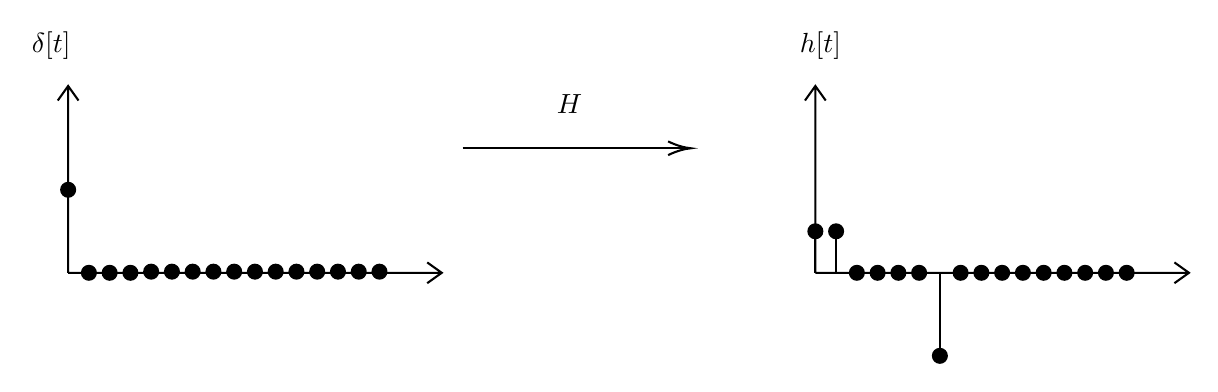
\begin{tikzpicture}[x=0.75pt,y=0.75pt,yscale=-1,xscale=1]
%uncomment if require: \path (0,300); %set diagram left start at 0, and has height of 300

%Shape: Axis 2D [id:dp8769733745764099] 
\draw  (70,170) -- (250,170)(70,80) -- (70,170) -- cycle (243,165) -- (250,170) -- (243,175) (65,87) -- (70,80) -- (75,87)  ;
%Straight Lines [id:da9568279078193335] 
\draw    (70,170) -- (70,130) ;
\draw [shift={(70,130)}, rotate = 270] [color={rgb, 255:red, 0; green, 0; blue, 0 }  ][fill={rgb, 255:red, 0; green, 0; blue, 0 }  ][line width=0.75]      (0, 0) circle [x radius= 3.35, y radius= 3.35]   ;
%Straight Lines [id:da3107691921176484] 
\draw    (260,110) -- (368,110) ;
\draw [shift={(370,110)}, rotate = 180] [color={rgb, 255:red, 0; green, 0; blue, 0 }  ][line width=0.75]    (10.93,-3.29) .. controls (6.95,-1.4) and (3.31,-0.3) .. (0,0) .. controls (3.31,0.3) and (6.95,1.4) .. (10.93,3.29)   ;
%Straight Lines [id:da4922161750710603] 
\draw    (80,170) ;
\draw [shift={(80,170)}, rotate = 0] [color={rgb, 255:red, 0; green, 0; blue, 0 }  ][fill={rgb, 255:red, 0; green, 0; blue, 0 }  ][line width=0.75]      (0, 0) circle [x radius= 3.35, y radius= 3.35]   ;
%Straight Lines [id:da26529554987645476] 
\draw    (90,170) ;
\draw [shift={(90,170)}, rotate = 0] [color={rgb, 255:red, 0; green, 0; blue, 0 }  ][fill={rgb, 255:red, 0; green, 0; blue, 0 }  ][line width=0.75]      (0, 0) circle [x radius= 3.35, y radius= 3.35]   ;
%Straight Lines [id:da32069114562205503] 
\draw    (100,170) ;
\draw [shift={(100,170)}, rotate = 0] [color={rgb, 255:red, 0; green, 0; blue, 0 }  ][fill={rgb, 255:red, 0; green, 0; blue, 0 }  ][line width=0.75]      (0, 0) circle [x radius= 3.35, y radius= 3.35]   ;
%Straight Lines [id:da6719768848433775] 
\draw    (110,170) -- (110,169.45) ;
\draw [shift={(110,169.45)}, rotate = 270] [color={rgb, 255:red, 0; green, 0; blue, 0 }  ][fill={rgb, 255:red, 0; green, 0; blue, 0 }  ][line width=0.75]      (0, 0) circle [x radius= 3.35, y radius= 3.35]   ;
%Straight Lines [id:da7882039258204357] 
\draw    (120,170) -- (120,169.45) ;
\draw [shift={(120,169.45)}, rotate = 270] [color={rgb, 255:red, 0; green, 0; blue, 0 }  ][fill={rgb, 255:red, 0; green, 0; blue, 0 }  ][line width=0.75]      (0, 0) circle [x radius= 3.35, y radius= 3.35]   ;
%Straight Lines [id:da037229806819463085] 
\draw    (130,170) -- (130,169.45) ;
\draw [shift={(130,169.45)}, rotate = 270] [color={rgb, 255:red, 0; green, 0; blue, 0 }  ][fill={rgb, 255:red, 0; green, 0; blue, 0 }  ][line width=0.75]      (0, 0) circle [x radius= 3.35, y radius= 3.35]   ;
%Straight Lines [id:da5004943871613776] 
\draw    (140,170) -- (140,169.45) ;
\draw [shift={(140,169.45)}, rotate = 270] [color={rgb, 255:red, 0; green, 0; blue, 0 }  ][fill={rgb, 255:red, 0; green, 0; blue, 0 }  ][line width=0.75]      (0, 0) circle [x radius= 3.35, y radius= 3.35]   ;
%Straight Lines [id:da21241757050344767] 
\draw    (150,170) -- (150,169.45) ;
\draw [shift={(150,169.45)}, rotate = 270] [color={rgb, 255:red, 0; green, 0; blue, 0 }  ][fill={rgb, 255:red, 0; green, 0; blue, 0 }  ][line width=0.75]      (0, 0) circle [x radius= 3.35, y radius= 3.35]   ;
%Straight Lines [id:da05053643331703561] 
\draw    (160,170) -- (160,169.45) ;
\draw [shift={(160,169.45)}, rotate = 270] [color={rgb, 255:red, 0; green, 0; blue, 0 }  ][fill={rgb, 255:red, 0; green, 0; blue, 0 }  ][line width=0.75]      (0, 0) circle [x radius= 3.35, y radius= 3.35]   ;
%Straight Lines [id:da0737208903849178] 
\draw    (170,170) -- (170,169.45) ;
\draw [shift={(170,169.45)}, rotate = 270] [color={rgb, 255:red, 0; green, 0; blue, 0 }  ][fill={rgb, 255:red, 0; green, 0; blue, 0 }  ][line width=0.75]      (0, 0) circle [x radius= 3.35, y radius= 3.35]   ;
%Straight Lines [id:da8623337053399087] 
\draw    (180,170) -- (180,169.45) ;
\draw [shift={(180,169.45)}, rotate = 270] [color={rgb, 255:red, 0; green, 0; blue, 0 }  ][fill={rgb, 255:red, 0; green, 0; blue, 0 }  ][line width=0.75]      (0, 0) circle [x radius= 3.35, y radius= 3.35]   ;
%Straight Lines [id:da37941330573195764] 
\draw    (190,170) -- (190,169.45) ;
\draw [shift={(190,169.45)}, rotate = 270] [color={rgb, 255:red, 0; green, 0; blue, 0 }  ][fill={rgb, 255:red, 0; green, 0; blue, 0 }  ][line width=0.75]      (0, 0) circle [x radius= 3.35, y radius= 3.35]   ;
%Straight Lines [id:da8358515707793517] 
\draw    (200,170) -- (200,169.45) ;
\draw [shift={(200,169.45)}, rotate = 270] [color={rgb, 255:red, 0; green, 0; blue, 0 }  ][fill={rgb, 255:red, 0; green, 0; blue, 0 }  ][line width=0.75]      (0, 0) circle [x radius= 3.35, y radius= 3.35]   ;
%Straight Lines [id:da9226938086822392] 
\draw    (210,170) -- (210,169.45) ;
\draw [shift={(210,169.45)}, rotate = 270] [color={rgb, 255:red, 0; green, 0; blue, 0 }  ][fill={rgb, 255:red, 0; green, 0; blue, 0 }  ][line width=0.75]      (0, 0) circle [x radius= 3.35, y radius= 3.35]   ;
%Straight Lines [id:da8194321549697962] 
\draw    (220,170) -- (220,169.45) ;
\draw [shift={(220,169.45)}, rotate = 270] [color={rgb, 255:red, 0; green, 0; blue, 0 }  ][fill={rgb, 255:red, 0; green, 0; blue, 0 }  ][line width=0.75]      (0, 0) circle [x radius= 3.35, y radius= 3.35]   ;
%Shape: Axis 2D [id:dp09196519122816926] 
\draw  (430,170) -- (610,170)(430,80) -- (430,170) -- cycle (603,165) -- (610,170) -- (603,175) (425,87) -- (430,80) -- (435,87)  ;
%Straight Lines [id:da39493540536245086] 
\draw    (430,170) -- (430,150) ;
\draw [shift={(430,150)}, rotate = 270] [color={rgb, 255:red, 0; green, 0; blue, 0 }  ][fill={rgb, 255:red, 0; green, 0; blue, 0 }  ][line width=0.75]      (0, 0) circle [x radius= 3.35, y radius= 3.35]   ;
%Straight Lines [id:da11139621857204629] 
\draw    (440,170) -- (440,150) ;
\draw [shift={(440,150)}, rotate = 270] [color={rgb, 255:red, 0; green, 0; blue, 0 }  ][fill={rgb, 255:red, 0; green, 0; blue, 0 }  ][line width=0.75]      (0, 0) circle [x radius= 3.35, y radius= 3.35]   ;
%Straight Lines [id:da8874688963653673] 
\draw    (450,170) ;
\draw [shift={(450,170)}, rotate = 0] [color={rgb, 255:red, 0; green, 0; blue, 0 }  ][fill={rgb, 255:red, 0; green, 0; blue, 0 }  ][line width=0.75]      (0, 0) circle [x radius= 3.35, y radius= 3.35]   ;
%Straight Lines [id:da7593740309454025] 
\draw    (460,170) ;
\draw [shift={(460,170)}, rotate = 0] [color={rgb, 255:red, 0; green, 0; blue, 0 }  ][fill={rgb, 255:red, 0; green, 0; blue, 0 }  ][line width=0.75]      (0, 0) circle [x radius= 3.35, y radius= 3.35]   ;
%Straight Lines [id:da1773320910071573] 
\draw    (470,170) ;
\draw [shift={(470,170)}, rotate = 0] [color={rgb, 255:red, 0; green, 0; blue, 0 }  ][fill={rgb, 255:red, 0; green, 0; blue, 0 }  ][line width=0.75]      (0, 0) circle [x radius= 3.35, y radius= 3.35]   ;
%Straight Lines [id:da3520401700293554] 
\draw    (480,170) ;
\draw [shift={(480,170)}, rotate = 0] [color={rgb, 255:red, 0; green, 0; blue, 0 }  ][fill={rgb, 255:red, 0; green, 0; blue, 0 }  ][line width=0.75]      (0, 0) circle [x radius= 3.35, y radius= 3.35]   ;
%Straight Lines [id:da5747485160635611] 
\draw    (490,170) -- (490,210) ;
\draw [shift={(490,210)}, rotate = 90] [color={rgb, 255:red, 0; green, 0; blue, 0 }  ][fill={rgb, 255:red, 0; green, 0; blue, 0 }  ][line width=0.75]      (0, 0) circle [x radius= 3.35, y radius= 3.35]   ;
%Straight Lines [id:da274017790334968] 
\draw    (500,170) ;
\draw [shift={(500,170)}, rotate = 0] [color={rgb, 255:red, 0; green, 0; blue, 0 }  ][fill={rgb, 255:red, 0; green, 0; blue, 0 }  ][line width=0.75]      (0, 0) circle [x radius= 3.35, y radius= 3.35]   ;
%Straight Lines [id:da6946786200443638] 
\draw    (510,170) ;
\draw [shift={(510,170)}, rotate = 0] [color={rgb, 255:red, 0; green, 0; blue, 0 }  ][fill={rgb, 255:red, 0; green, 0; blue, 0 }  ][line width=0.75]      (0, 0) circle [x radius= 3.35, y radius= 3.35]   ;
%Straight Lines [id:da22256573907165378] 
\draw    (520,170) ;
\draw [shift={(520,170)}, rotate = 0] [color={rgb, 255:red, 0; green, 0; blue, 0 }  ][fill={rgb, 255:red, 0; green, 0; blue, 0 }  ][line width=0.75]      (0, 0) circle [x radius= 3.35, y radius= 3.35]   ;
%Straight Lines [id:da4080213070412726] 
\draw    (530,170) ;
\draw [shift={(530,170)}, rotate = 0] [color={rgb, 255:red, 0; green, 0; blue, 0 }  ][fill={rgb, 255:red, 0; green, 0; blue, 0 }  ][line width=0.75]      (0, 0) circle [x radius= 3.35, y radius= 3.35]   ;
%Straight Lines [id:da39273440022231276] 
\draw    (540,170) ;
\draw [shift={(540,170)}, rotate = 0] [color={rgb, 255:red, 0; green, 0; blue, 0 }  ][fill={rgb, 255:red, 0; green, 0; blue, 0 }  ][line width=0.75]      (0, 0) circle [x radius= 3.35, y radius= 3.35]   ;
%Straight Lines [id:da03964806427023371] 
\draw    (550,170) ;
\draw [shift={(550,170)}, rotate = 0] [color={rgb, 255:red, 0; green, 0; blue, 0 }  ][fill={rgb, 255:red, 0; green, 0; blue, 0 }  ][line width=0.75]      (0, 0) circle [x radius= 3.35, y radius= 3.35]   ;
%Straight Lines [id:da5419692471474935] 
\draw    (560,170) ;
\draw [shift={(560,170)}, rotate = 0] [color={rgb, 255:red, 0; green, 0; blue, 0 }  ][fill={rgb, 255:red, 0; green, 0; blue, 0 }  ][line width=0.75]      (0, 0) circle [x radius= 3.35, y radius= 3.35]   ;
%Straight Lines [id:da5734589283089392] 
\draw    (570,170) ;
\draw [shift={(570,170)}, rotate = 0] [color={rgb, 255:red, 0; green, 0; blue, 0 }  ][fill={rgb, 255:red, 0; green, 0; blue, 0 }  ][line width=0.75]      (0, 0) circle [x radius= 3.35, y radius= 3.35]   ;
%Straight Lines [id:da6012285540274246] 
\draw    (580,170) ;
\draw [shift={(580,170)}, rotate = 0] [color={rgb, 255:red, 0; green, 0; blue, 0 }  ][fill={rgb, 255:red, 0; green, 0; blue, 0 }  ][line width=0.75]      (0, 0) circle [x radius= 3.35, y radius= 3.35]   ;

% Text Node
\draw (51,52.4) node [anchor=north west][inner sep=0.75pt]    {$\delta [ t]$};
% Text Node
\draw (421,52.4) node [anchor=north west][inner sep=0.75pt]    {$h[ t]$};
% Text Node
\draw (304,82.4) node [anchor=north west][inner sep=0.75pt]    {$H$};


\end{tikzpicture}
\end{center}
Since any input signal is a sum of scaled and shifted delta functions, applying an 
LTI system to an input signal is equivalent to taking the corresponding scalings and 
shifts of the impulse response and adding them together. 
Thus an LTI system can be completely described by its impulse response.

\begin{center}

\tikzset{every picture/.style={line width=0.75pt}} %set default line width to 0.75pt        

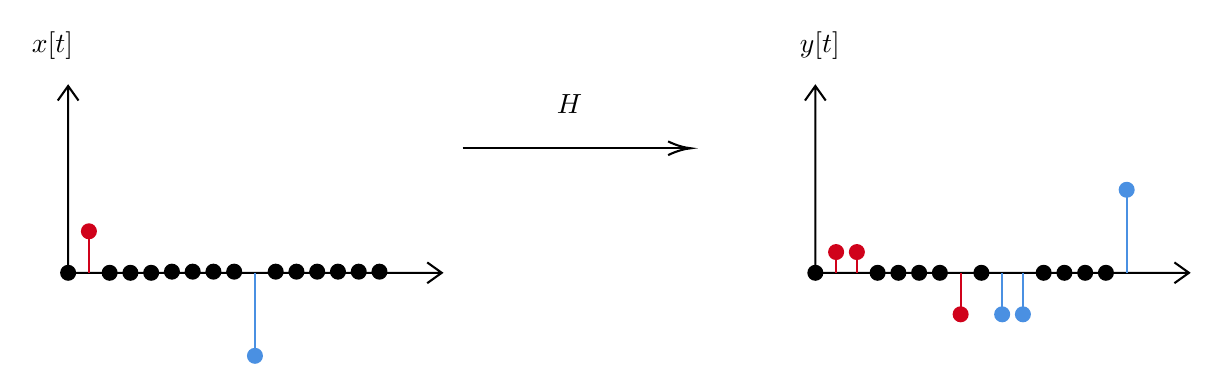
\begin{tikzpicture}[x=0.75pt,y=0.75pt,yscale=-1,xscale=1]
%uncomment if require: \path (0,300); %set diagram left start at 0, and has height of 300

%Shape: Axis 2D [id:dp791354747049518] 
\draw  (60,170) -- (240,170)(60,80) -- (60,170) -- cycle (233,165) -- (240,170) -- (233,175) (55,87) -- (60,80) -- (65,87)  ;
%Straight Lines [id:da5046356363776592] 
\draw    (60,170) ;
\draw [shift={(60,170)}, rotate = 0] [color={rgb, 255:red, 0; green, 0; blue, 0 }  ][fill={rgb, 255:red, 0; green, 0; blue, 0 }  ][line width=0.75]      (0, 0) circle [x radius= 3.35, y radius= 3.35]   ;
%Straight Lines [id:da9809158048232325] 
\draw    (250,110) -- (358,110) ;
\draw [shift={(360,110)}, rotate = 180] [color={rgb, 255:red, 0; green, 0; blue, 0 }  ][line width=0.75]    (10.93,-3.29) .. controls (6.95,-1.4) and (3.31,-0.3) .. (0,0) .. controls (3.31,0.3) and (6.95,1.4) .. (10.93,3.29)   ;
%Straight Lines [id:da9981205777005407] 
\draw [color={rgb, 255:red, 208; green, 2; blue, 27 }  ,draw opacity=1 ]   (70,170) -- (70,150) ;
\draw [shift={(70,150)}, rotate = 270] [color={rgb, 255:red, 208; green, 2; blue, 27 }  ,draw opacity=1 ][fill={rgb, 255:red, 208; green, 2; blue, 27 }  ,fill opacity=1 ][line width=0.75]      (0, 0) circle [x radius= 3.35, y radius= 3.35]   ;
%Straight Lines [id:da8385320667815575] 
\draw    (80,170) ;
\draw [shift={(80,170)}, rotate = 0] [color={rgb, 255:red, 0; green, 0; blue, 0 }  ][fill={rgb, 255:red, 0; green, 0; blue, 0 }  ][line width=0.75]      (0, 0) circle [x radius= 3.35, y radius= 3.35]   ;
%Straight Lines [id:da14277617185264935] 
\draw    (90,170) ;
\draw [shift={(90,170)}, rotate = 0] [color={rgb, 255:red, 0; green, 0; blue, 0 }  ][fill={rgb, 255:red, 0; green, 0; blue, 0 }  ][line width=0.75]      (0, 0) circle [x radius= 3.35, y radius= 3.35]   ;
%Straight Lines [id:da7250456445117891] 
\draw    (100,170) ;
\draw [shift={(100,170)}, rotate = 0] [color={rgb, 255:red, 0; green, 0; blue, 0 }  ][fill={rgb, 255:red, 0; green, 0; blue, 0 }  ][line width=0.75]      (0, 0) circle [x radius= 3.35, y radius= 3.35]   ;
%Straight Lines [id:da4466348586781691] 
\draw    (110,170) -- (110,169.45) ;
\draw [shift={(110,169.45)}, rotate = 270] [color={rgb, 255:red, 0; green, 0; blue, 0 }  ][fill={rgb, 255:red, 0; green, 0; blue, 0 }  ][line width=0.75]      (0, 0) circle [x radius= 3.35, y radius= 3.35]   ;
%Straight Lines [id:da4165334374839318] 
\draw    (120,170) -- (120,169.45) ;
\draw [shift={(120,169.45)}, rotate = 270] [color={rgb, 255:red, 0; green, 0; blue, 0 }  ][fill={rgb, 255:red, 0; green, 0; blue, 0 }  ][line width=0.75]      (0, 0) circle [x radius= 3.35, y radius= 3.35]   ;
%Straight Lines [id:da7195990046641679] 
\draw    (130,170) -- (130,169.45) ;
\draw [shift={(130,169.45)}, rotate = 270] [color={rgb, 255:red, 0; green, 0; blue, 0 }  ][fill={rgb, 255:red, 0; green, 0; blue, 0 }  ][line width=0.75]      (0, 0) circle [x radius= 3.35, y radius= 3.35]   ;
%Straight Lines [id:da07287453114767628] 
\draw    (140,170) -- (140,169.45) ;
\draw [shift={(140,169.45)}, rotate = 270] [color={rgb, 255:red, 0; green, 0; blue, 0 }  ][fill={rgb, 255:red, 0; green, 0; blue, 0 }  ][line width=0.75]      (0, 0) circle [x radius= 3.35, y radius= 3.35]   ;
%Straight Lines [id:da25954389536811406] 
\draw [color={rgb, 255:red, 74; green, 144; blue, 226 }  ,draw opacity=1 ]   (150,170) -- (150,210) ;
\draw [shift={(150,210)}, rotate = 90] [color={rgb, 255:red, 74; green, 144; blue, 226 }  ,draw opacity=1 ][fill={rgb, 255:red, 74; green, 144; blue, 226 }  ,fill opacity=1 ][line width=0.75]      (0, 0) circle [x radius= 3.35, y radius= 3.35]   ;
%Straight Lines [id:da8079272840506293] 
\draw    (160,170) -- (160,169.45) ;
\draw [shift={(160,169.45)}, rotate = 270] [color={rgb, 255:red, 0; green, 0; blue, 0 }  ][fill={rgb, 255:red, 0; green, 0; blue, 0 }  ][line width=0.75]      (0, 0) circle [x radius= 3.35, y radius= 3.35]   ;
%Straight Lines [id:da5521681935908768] 
\draw    (170,170) -- (170,169.45) ;
\draw [shift={(170,169.45)}, rotate = 270] [color={rgb, 255:red, 0; green, 0; blue, 0 }  ][fill={rgb, 255:red, 0; green, 0; blue, 0 }  ][line width=0.75]      (0, 0) circle [x radius= 3.35, y radius= 3.35]   ;
%Straight Lines [id:da46511016308207775] 
\draw    (180,170) -- (180,169.45) ;
\draw [shift={(180,169.45)}, rotate = 270] [color={rgb, 255:red, 0; green, 0; blue, 0 }  ][fill={rgb, 255:red, 0; green, 0; blue, 0 }  ][line width=0.75]      (0, 0) circle [x radius= 3.35, y radius= 3.35]   ;
%Straight Lines [id:da4346176203359218] 
\draw    (190,170) -- (190,169.45) ;
\draw [shift={(190,169.45)}, rotate = 270] [color={rgb, 255:red, 0; green, 0; blue, 0 }  ][fill={rgb, 255:red, 0; green, 0; blue, 0 }  ][line width=0.75]      (0, 0) circle [x radius= 3.35, y radius= 3.35]   ;
%Straight Lines [id:da2679112607227163] 
\draw    (200,170) -- (200,169.45) ;
\draw [shift={(200,169.45)}, rotate = 270] [color={rgb, 255:red, 0; green, 0; blue, 0 }  ][fill={rgb, 255:red, 0; green, 0; blue, 0 }  ][line width=0.75]      (0, 0) circle [x radius= 3.35, y radius= 3.35]   ;
%Straight Lines [id:da43142319482023705] 
\draw    (210,170) -- (210,169.45) ;
\draw [shift={(210,169.45)}, rotate = 270] [color={rgb, 255:red, 0; green, 0; blue, 0 }  ][fill={rgb, 255:red, 0; green, 0; blue, 0 }  ][line width=0.75]      (0, 0) circle [x radius= 3.35, y radius= 3.35]   ;
%Shape: Axis 2D [id:dp7345401677189357] 
\draw  (420,170) -- (600,170)(420,80) -- (420,170) -- cycle (593,165) -- (600,170) -- (593,175) (415,87) -- (420,80) -- (425,87)  ;
%Straight Lines [id:da23914075749417785] 
\draw    (420,170) ;
\draw [shift={(420,170)}, rotate = 0] [color={rgb, 255:red, 0; green, 0; blue, 0 }  ][fill={rgb, 255:red, 0; green, 0; blue, 0 }  ][line width=0.75]      (0, 0) circle [x radius= 3.35, y radius= 3.35]   ;
%Straight Lines [id:da9129442704941363] 
\draw [color={rgb, 255:red, 208; green, 2; blue, 27 }  ,draw opacity=1 ]   (430,170) -- (430,160) ;
\draw [shift={(430,160)}, rotate = 270] [color={rgb, 255:red, 208; green, 2; blue, 27 }  ,draw opacity=1 ][fill={rgb, 255:red, 208; green, 2; blue, 27 }  ,fill opacity=1 ][line width=0.75]      (0, 0) circle [x radius= 3.35, y radius= 3.35]   ;
%Straight Lines [id:da7870382784710074] 
\draw [color={rgb, 255:red, 208; green, 2; blue, 27 }  ,draw opacity=1 ]   (440,170) -- (440,160) ;
\draw [shift={(440,160)}, rotate = 270] [color={rgb, 255:red, 208; green, 2; blue, 27 }  ,draw opacity=1 ][fill={rgb, 255:red, 208; green, 2; blue, 27 }  ,fill opacity=1 ][line width=0.75]      (0, 0) circle [x radius= 3.35, y radius= 3.35]   ;
%Straight Lines [id:da27232922247850566] 
\draw    (450,170) ;
\draw [shift={(450,170)}, rotate = 0] [color={rgb, 255:red, 0; green, 0; blue, 0 }  ][fill={rgb, 255:red, 0; green, 0; blue, 0 }  ][line width=0.75]      (0, 0) circle [x radius= 3.35, y radius= 3.35]   ;
%Straight Lines [id:da8995478110988177] 
\draw    (460,170) ;
\draw [shift={(460,170)}, rotate = 0] [color={rgb, 255:red, 0; green, 0; blue, 0 }  ][fill={rgb, 255:red, 0; green, 0; blue, 0 }  ][line width=0.75]      (0, 0) circle [x radius= 3.35, y radius= 3.35]   ;
%Straight Lines [id:da7889414111887794] 
\draw    (470,170) ;
\draw [shift={(470,170)}, rotate = 0] [color={rgb, 255:red, 0; green, 0; blue, 0 }  ][fill={rgb, 255:red, 0; green, 0; blue, 0 }  ][line width=0.75]      (0, 0) circle [x radius= 3.35, y radius= 3.35]   ;
%Straight Lines [id:da8575968668358517] 
\draw    (480,170) ;
\draw [shift={(480,170)}, rotate = 0] [color={rgb, 255:red, 0; green, 0; blue, 0 }  ][fill={rgb, 255:red, 0; green, 0; blue, 0 }  ][line width=0.75]      (0, 0) circle [x radius= 3.35, y radius= 3.35]   ;
%Straight Lines [id:da3692513436275784] 
\draw [color={rgb, 255:red, 208; green, 2; blue, 27 }  ,draw opacity=1 ]   (490,170) -- (490,190) ;
\draw [shift={(490,190)}, rotate = 90] [color={rgb, 255:red, 208; green, 2; blue, 27 }  ,draw opacity=1 ][fill={rgb, 255:red, 208; green, 2; blue, 27 }  ,fill opacity=1 ][line width=0.75]      (0, 0) circle [x radius= 3.35, y radius= 3.35]   ;
%Straight Lines [id:da5692450340598083] 
\draw    (500,170) ;
\draw [shift={(500,170)}, rotate = 0] [color={rgb, 255:red, 0; green, 0; blue, 0 }  ][fill={rgb, 255:red, 0; green, 0; blue, 0 }  ][line width=0.75]      (0, 0) circle [x radius= 3.35, y radius= 3.35]   ;
%Straight Lines [id:da2834829347441865] 
\draw [color={rgb, 255:red, 74; green, 144; blue, 226 }  ,draw opacity=1 ]   (510,170) -- (510,190) ;
\draw [shift={(510,190)}, rotate = 90] [color={rgb, 255:red, 74; green, 144; blue, 226 }  ,draw opacity=1 ][fill={rgb, 255:red, 74; green, 144; blue, 226 }  ,fill opacity=1 ][line width=0.75]      (0, 0) circle [x radius= 3.35, y radius= 3.35]   ;
%Straight Lines [id:da2980766617642864] 
\draw [color={rgb, 255:red, 74; green, 144; blue, 226 }  ,draw opacity=1 ]   (520,170) -- (520,190) ;
\draw [shift={(520,190)}, rotate = 90] [color={rgb, 255:red, 74; green, 144; blue, 226 }  ,draw opacity=1 ][fill={rgb, 255:red, 74; green, 144; blue, 226 }  ,fill opacity=1 ][line width=0.75]      (0, 0) circle [x radius= 3.35, y radius= 3.35]   ;
%Straight Lines [id:da3440488095668025] 
\draw    (530,170) ;
\draw [shift={(530,170)}, rotate = 0] [color={rgb, 255:red, 0; green, 0; blue, 0 }  ][fill={rgb, 255:red, 0; green, 0; blue, 0 }  ][line width=0.75]      (0, 0) circle [x radius= 3.35, y radius= 3.35]   ;
%Straight Lines [id:da34245358635452783] 
\draw    (540,170) ;
\draw [shift={(540,170)}, rotate = 0] [color={rgb, 255:red, 0; green, 0; blue, 0 }  ][fill={rgb, 255:red, 0; green, 0; blue, 0 }  ][line width=0.75]      (0, 0) circle [x radius= 3.35, y radius= 3.35]   ;
%Straight Lines [id:da5967606319976225] 
\draw    (550,170) ;
\draw [shift={(550,170)}, rotate = 0] [color={rgb, 255:red, 0; green, 0; blue, 0 }  ][fill={rgb, 255:red, 0; green, 0; blue, 0 }  ][line width=0.75]      (0, 0) circle [x radius= 3.35, y radius= 3.35]   ;
%Straight Lines [id:da35562519265748127] 
\draw    (560,170) ;
\draw [shift={(560,170)}, rotate = 0] [color={rgb, 255:red, 0; green, 0; blue, 0 }  ][fill={rgb, 255:red, 0; green, 0; blue, 0 }  ][line width=0.75]      (0, 0) circle [x radius= 3.35, y radius= 3.35]   ;
%Straight Lines [id:da7651679932280698] 
\draw [color={rgb, 255:red, 74; green, 144; blue, 226 }  ,draw opacity=1 ]   (570,170) -- (570,130) ;
\draw [shift={(570,130)}, rotate = 270] [color={rgb, 255:red, 74; green, 144; blue, 226 }  ,draw opacity=1 ][fill={rgb, 255:red, 74; green, 144; blue, 226 }  ,fill opacity=1 ][line width=0.75]      (0, 0) circle [x radius= 3.35, y radius= 3.35]   ;

% Text Node
\draw (41,52.4) node [anchor=north west][inner sep=0.75pt]    {$x[ t]$};
% Text Node
\draw (411,52.4) node [anchor=north west][inner sep=0.75pt]    {$y[ t]$};
% Text Node
\draw (294,82.4) node [anchor=north west][inner sep=0.75pt]    {$H$};


\end{tikzpicture}
\end{center}

Thus it's easy to see that applying an LTI system onto a signal is equivalent to 
convolving the signal with the impulse response of the system.

\subsection{Response of Sinusoids}
When a sinusoid is fed through an LTI system, the output signal is also sinusoidal,
with the same frequency, but different amplitude and phase.

$$y[t]=\sum_{i=0}^n h[i]x[t-i]$$

Since the term on the right is the sum of sinusoids of equal frequency,
the resulting output signal is also a sinusoid with the same frequency.

Sinusoids of different frequencies $\omega$ (measured in radians per sample) which are fed into the same LTI filter
may have their amplitudes (and phases) affected differently. 
For every $\omega$ that corresponds to a frequency bin in the DFT, 
the frequency response at $\omega$ is equal to the output amplitude when the input
is a sinusoid with frequency $\omega$ and amplitude $1$.

\pagebreak

\subsection{Discrete-Time Fourier Transform}
Unlike the DFT which can only be evaluated at certain frequences, 
the DTFT gives a function that can be evaluated at any frequency $\omega$ (measured in radians per sample) on the continuous spectrum.
$$DFT\left[\frac{n\omega}{2\pi}\right]=\sum_{t=0}^nx[t]e^{-i\omega t}$$
$$DTFT(e^{i\omega})=\sum_{t=0}^nx[t]e^{-i\omega t}$$

The DFT is essentially the DTFT sampled at the specific frequencies (1 to N/2 cycles per window).

\subsection{Frequency Response}
The frequency response of a LTI system as a function of frequency $\omega$ is equal
to the amount that the amplitude of a sinusoid with frequency $\omega$ would be scaled by when fed through the system.
The frequency response of the system is equal to the DTFT of the impulse response,
taking the magnitude of each phasor.

This is because convolving a signal with the impulse response (convolution in the time domain)
is equivalent to performing component-wise multiplication of the DFT of the signal with the DFT of the impulse response.
Therefore the DFT of the impulse response represents how much each frequency component of the signal will be scaled by
when the LTI system is applied.

This comes from the discrete version of the convolution theorem.

This can be generalised, where the frequency response can be calculated for continuous $\omega$ values 
not necessarily corresponding to any DFT frequency bin. This is just done using the DTFT.

\subsection{Filter Design}
Instead of using a system's impulse response to find its frequency response, 
you can use a desired frequency response and perform an IDFT to produce the 
kernel for a system that has that desired frequency response.

However for the purpose of making this implementation easier, I will just use 
perform low pass filtering using a moving average. A moving average will 
tend to attenuate high frequencies. A corresponding high pass filter kernel can be
produced by using linearity properties.

The moving average uses a rectangular kernel.
The frequency response of this filter can be found by using the DTFT of the rectangular kernel.
\pagebreak 

Suppose that the length of the rectangular kernel is $W$ samples. 
In other words, the kernel is $h$, where $h[t]=\frac{1}{W}$ for $0\leq t < W$, and $h[t]=0$ everywhere else.
Finding the DTFT of the kernel:
\begin{align*}
    DTFT(e^{i\omega})
    &= \sum_{t=0}^n h[t] e^{-i\omega t}\\
    &= \frac{1}{W} \sum_{t=0}^W e^{-i\omega t}\\
    &= \frac{1}{W} \frac{1-e^{-i\omega W }}{1-e^{i\omega }}\\
    &= \frac{1}{W} \frac{e^{-i\omega W /2}(e^{i\omega W /2}-e^{-i\omega W /2})}{e^{-i\omega t/2}(e^{i\omega /2}-e^{-i\omega /2})}\\
    &= \frac{1}{W} e^{-i\omega (W-1) /2} \frac{\sin (\omega W /2)}{\sin (\omega /2)}
\end{align*}

Taking the magnitude of both sides to find the frequency magnitude response gives
$$|DTFT(e^{i\omega})|=\frac{1}{W}\left|\frac{\sin (\omega W /2)}{\sin (\omega /2)}\right|$$

Below is a graph of the frequency magnitude response vs frequency (radians per sample).
The green graph is when $W=6$ and the red graph is when $W=5$.
\begin{center}\includegraphics[height=4cm]{assets/rectangledtft.png}\end{center}

As expected, in both cases, high frequencies are attenuated.
Also the wider the rectangle, the thinner the lobe of the frequency magnitude response,
thus less high frequencies are let through.

\pagebreak

\subsection{Implementation}
This time the FFT will be used to perform a convolution of the windowed input signal
with the kernel.

For these, I made new \verb|WindowProcessor| functor subclasses.
The first is the \verb|FConvLowpass| subclass.

\begin{verbatim}
struct FConvLowpass : public WindowProcessor {
    size_t width_;
    Transformer transformer_;
    std::vector<std::complex<double>> kernel_;

    FConvLowpass(size_t width, size_t win_size);

    std::vector<std::complex<double>> operator()(
        std::vector<std::complex<double>> const& signal
    ) override;
};
\end{verbatim}

This class is constructed with a \verb|win_size| parameter.
During the construction, the kernel vector is populated:

\begin{verbatim}
FConvLowpass::FConvLowpass(size_t width, size_t win_size) : 
width_(width), transformer_(win_size), kernel_(win_size, 0) {
    for (int i = 0; i < width; ++i) {
        kernel_[i] = 1/((double) width);
    }
}
\end{verbatim}

Throughout the lifetime of a \verb|FConvLowpass| object, 
this kernel vector is not modified.
Therefore we do not need to construct and populate a new kernel vector 
every time we want to perform a convolution.

Like all other \verb|WindowProcessor| objects, the address of a
\verb|FConvLowpass| object is passed in during the construction of a
\verb|StreamProcessor| object (dependency injection).
As audio data is inserted into the stream, this results in the
function call operator being called:

\begin{verbatim}
    // then process it using the window processing functor
    auto processed_window = win_processor->operator()(window);
\end{verbatim}

The \verb|FConvLowpass| class overrides the function call operator as shown below.

\begin{verbatim}
std::vector<std::complex<double>> FConvLowpass::operator()(
    std::vector<std::complex<double>> const& signal
) {
    return convolve(signal, kernel_, transformer_);
}
\end{verbatim}

\pagebreak

The convolve function takes two vectors of complex doubles of the same length.
Then it performs DFTs on both of them.
After this it performs component-wise multiplication, before finally
performing an IDFT to return the result of the convolution.

\begin{verbatim}
std::vector<std::complex<double>> convolve(
    std::vector<std::complex<double>> const& signal,
    std::vector<std::complex<double>> const& kernel,
    Transformer const& t
) {
    int n = signal.size();
    auto dft_signal = t.dft(signal);
    auto dft_kernel = t.dft(kernel);

    // component-wise multiplication
    for (int i = 0; i < n; ++i) {
        dft_signal[i] *= dft_kernel[i];
    }

    return t.idft(dft_signal);
}
\end{verbatim}

The \verb|FConvLowpass| functor just uses a rectangular kernel to perform
a moving average. 
The \verb|FConvHighpass| functor uses a kernel which is just the same rectangular
kernel subtracted from the delta function.

\begin{verbatim}
FConvHighpass::FConvHighpass(size_t width, size_t win_size) 
: width_(width), transformer_(win_size), kernel_(win_size, 0) {
    for (int i = 0; i < width; ++i) {
        kernel_[i] = -1/((double) width);
    }
    kernel_[0] += 1;
}
\end{verbatim}

This works because the filter defined by this kernel is just the
low pass filter subtracted from the identity filter, 
meaning that the low frequencies are removed, only allowing high frequencies to pass.

This is possible because convolving with the sum of two kernels is
equivalent to performing separate convolutions with the kernels and then
adding the resulting signals together.
